%%=============================================================================
%% Methodologie
%%=============================================================================

\chapter{\IfLanguageName{dutch}{Methodologie}{Methodology}}
\label{ch:methodologie}

%% TODO: Hoe ben je te werk gegaan? Verdeel je onderzoek in grote fasen, en
%% licht in elke fase toe welke stappen je gevolgd hebt. Verantwoord waarom je
%% op deze manier te werk gegaan bent. Je moet kunnen aantonen dat je de best
%% mogelijke manier toegepast hebt om een antwoord te vinden op de
%% onderzoeksvraag.

In dit onderdeel wordt de methodologie van data mining en webscraping applicaties binnen de InsurTech geïllustreerd met beschrijvingen omtrent iedere fase.

\section{Opbouw van het onderzoek}
Voor dit onderzoek werd gewerkt met de vooraf omschreven tools en technieken.
Data die online werd verzameld werd verrijkt door irrelevante informatie eruit te filteren en te combineren met gelijksoortige informatie. Hierbij werd enkel de nuttige data overgehouden, die relevant was om bij te houden voor later in het onderzoek.
Een eerste fase binnen het onderzoek is een keuze maken welke categorie van de InsurTech precies onderzocht wordt. Het doel is om een prototype uit te werken waarin een toepassing van de InsurTech via webscraping wordt toegelicht.
In dit onderzoek werden verschillende fases doorlopen om tot informatieve en duidelijke conclusies en resultaten te komen aan de hand van bewijzen.

De eerste fase van het onderzoek omvatte een keuze maken tussen welke categorie In de InsurTech precies een prototype zou gemaakt worden. Het is hierbij van belang dat het mede onderwerp in deze in dit onderzoek "webscraping" zeker aan bod kwam. Een requirement waaraan de categorie zeker moest voldoen is dat de gescrapete data verwerkt zou worden publiekelijk beschikbaar was. 
Zo kan een web scraper deze data scrapen en deze efficiënt gebruiken binnen het prototype. 
Meer over de term "publiekelijk" werd in het onderzoek uitvoerig besproken.

Dit omvat dan ook de tweede fase van het onderzoek, een zoektocht naar een webpagina of webpagina's die gescrapet konden worden.
Op zoek naar webpagina's die relevante data bevatten werkt de zoekmachine Google gebruikt. Hierbij werd nagegaan per webpagina als er voldoende relevante data beschikbaar was.

De derde fase van het onderzoek omvatte op basis van de gekozen webpagina's een concreet plan opgestellen over hoe de webscraper stapsgewijs precies de nodige data uit de webpagina scrapet. Het was hierbij van belang dat de gescrapete - mogelijks ongestructureerde – data in een gestructureerd formaat werd gegoten.

\begin{figure}[H]
	\centering
	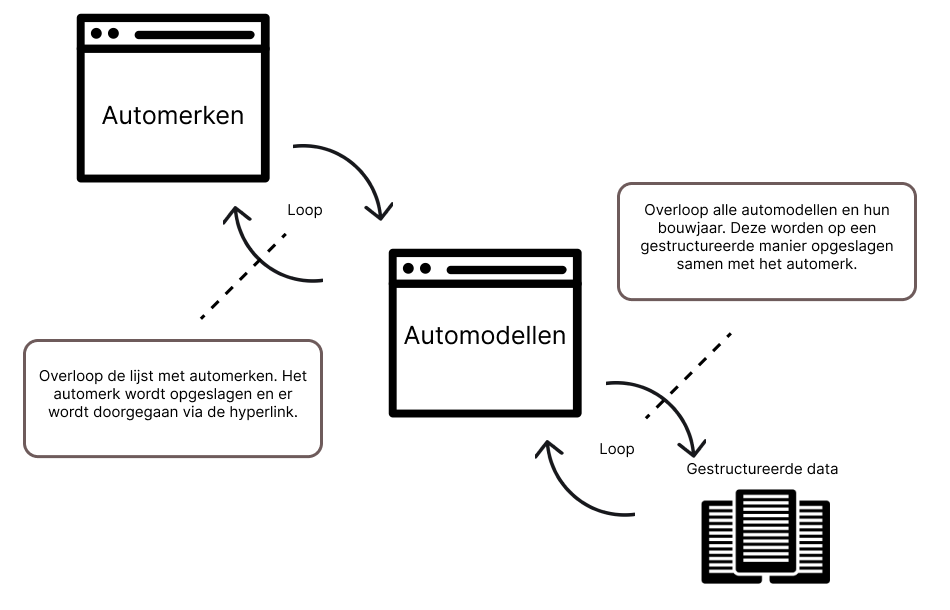
\includegraphics[width=\textwidth, height=\textheight, keepaspectratio]{car_info_webscraping_plan}
	\caption{Stapsgewijs scraping plan}
\end{figure}

Zo kwam ook aan bod welke hindernissen web scraper kan tegenkomen die data bevat die relevant kan zijn voor de InsurTech categorie. Eenmaal in deze categorie een proces werd gekozen, werden de verschillende stappen die het proces die het uitvoer proces omschrijven, opgelijst en omschreven.

De vierde fase van het onderzoek was aan de slag gaan met het schrijven van Python code volgens het omschreven plan, waarbij eerst en vooral data werd gescrapet, vervolgens opgeslagen en als laatste verwerkt in een simpele interactieve lay-out die toepassing hiermee moet voorstellen. In deze fase wordt de code uitvoerig en stapsgewijs beschreven, zodat deze gerepliceerd en begrepen kan worden. Hierbij zijn bijhorende codeblokken en screenshots van webpagina's toegevoegd.

Als laatste fase was het uiteraard van belang een analyse te doen van het prototype tegenover de "normale gang van zaken", waar InsurTech niet aan te pas komt. Hierbij werden feiten opgelijst uit de data die opgehaald werd, alsook wat precies de optimalisatie was.


